\documentclass[10pt,a4paper]{article}

%double si on veut une version prof et une version élève. simple si on veut une seule version.
\newcommand{\buildmode}{double}

\InputIfFileExists{version.tex}{}{}
% Version (définie par le script)
\providecommand{\version}{eleve}

\usepackage{feuilleexo}
\usepackage{schemaevolution}

%%%à modifier à chaque fois

\renewcommand{\niveau}{SBM 2A}
\renewcommand{\chapitre}{Probabilités}
\renewcommand{\numchap}{0.1} 
\renewcommand{\theme}{Probabilités}

\begin{document}


%\legendeicones

\vspace{-0.3cm}

\begin{prerequis}
\begin{itemize}
    \item Savoir calculer une proportion et la mettre sous différentes formes
    \item Comprendre une probabilité comme une notion du hasard
\end{itemize}

\end{prerequis}

\prof{
    Faire de la récupération sur les probabilités en début de cours. Séparer en deux parties.
}
\begin{multicols}{2}

\section{Probabilités conditionnelles}


\prof{
    À la fin de chaque exercice, on peut mettre une question de compréhension des probas.
}

\begin{exo}[][]
Voici un arbre de probabilité.

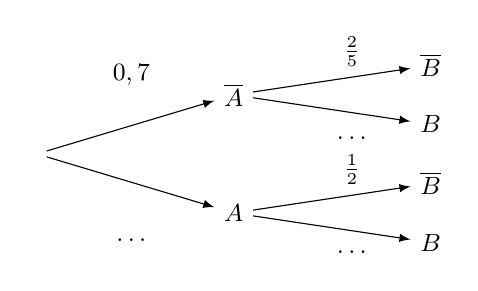
\begin{tikzpicture}[
    grow=right,
    level 1/.style={sibling distance=1.5cm, level distance=2.5cm},
    level 2/.style={sibling distance=0.75cm, level distance=2.5cm},
    every node/.style={font=\small},
    edge from parent/.style={draw, -latex},
]

% Premier niveau
\node {}
    child {
        node {$A$}
        child {
            node {$B$}
        }
        child {
            node {$\overline{B}$}
        }
    }
    child {
        node {$\overline{A}$}
        child {
            node {$B$}
        }
        child {
            node {$\overline{B}$}
        }
    };

% Probabilités du premier niveau
\node at (1.2,1) {$0,7$};
\node at (1.2,-1.1) {$\ldots$};

% Probabilités du deuxième niveau
\node at (4,1.3) {$\frac{2}{5}$};
\node at (4,0.2) {$\ldots$};
\node at (4,-0.2) {$\frac{1}{2}$};
\node at (4,-1.25) {$\ldots$};

\end{tikzpicture}

\begin{enumerate}
    \item Compléter cet arbre.
    \item Déterminer les probabilités suivantes : \(P(A)\), \(P(\overline{A})\), \(P_A(B)\), \(P_A(\overline{B})\).
    \item Déterminer \(P(B)\) puis \(P_B(A)\).
    \item Inventer une situation qui peut être modélisée par cet arbre.
\end{enumerate}
\end{exo}

\begin{exo}[][ccf]
    Dans un laboratoire de biologie médicale, on réalise une analyse sur des échantillons sanguins afin de rechercher la présence d'une anomalie biologique. 1000 échantillons ont été testés. \medskip
    On note A "Le test présente une anomalie" et T : "Le test est positif" \medskip
    Les résulats des échantillons sont reportés dans le tableau ci-dessous :
    \begin{tabular}{|C{0.07\textwidth}|C{0.1\textwidth}|C{0.1\textwidth}|C{0.07\textwidth}|}
        \hline
         & Présence d'anomalie ($A$) & Abscence d'anomalie ($\overline{A}$) & Total \\ \hline
         Test positif ($T$) & 80 & 100 & 180 \\
         \hline
        Test négatif ($\overline{T}$) & 20 & 900 & 920 \\ \hline
        Total & 100 & 900 & 1000 \\
        \hline
    \end{tabular}

    \begin{enumerate}
        \item \begin{enumerate}
            \item Calculer et interpréter $P(T)$, puis $P(A\cap T)$
            \item Calculer $P_T(A)$ et $P_{\overline{T}}(A)$. Interpréter.
            \item Construire un arbre de probabilité avec les probabilités calculées.
            \item Que constatez-vous ? Comment l'expliquez-vous ?
        \end{enumerate}
        \item \begin{enumerate}
            \item Calculer $P_A(T)$ et $P_{\overline{A}}(T)$
            \item En déduire un nouvel arbre de probabilité.
            \item Dans le contexte de vérification de l'efficacité du vaccin, est-il plus pertinent de connaître $P_A(T)$ ou $P_T(A)$ selon vous ?
        \end{enumerate}
    \end{enumerate}
\end{exo}

\section{Variables aléatoires}
\begin{exo}
Lors d'un contrôle qualité, un technicien vérifie successivement 10 échantillons. On considère que la probabilité qu'un échantillon soit conforme est de 0,95. Les contrôles sont supposés indépendants.

On note X le nombre d'échantillons \underline{non conformes} parmi les 10.

\begin{enumerate}
    \item Justifier que \(X\) suit une loi binomiale dont on précisera les paramètres.
    \item Calculer \(P(X=10)\). Interpréter.
    \item Calculer la probabilité d'avoir maximum 3 échantillons non conformes
    \item Déterminer \(E(X)\) et interpréter le résultat.
\end{enumerate}
\end{exo}

\begin{exo}[][]
    Dans une population donnée, la concentration (en mg/L) d'une substance dans le sang est modélisée par une variable aléatoire \(X\) suivant une loi normale de moyenne \(\mu = 100\) et d'écart-type \(\sigma = 12\).
    \begin{enumerate}
        \item Rappeler à quoi correspondent \(\mu\) et \(\sigma\).
        \item Calculer \(P(88\geq X\geq 112)\)
        \item Quelle est la probabilité qu'un individu ait une concentration supérieure à 124 mg/L ?
    \end{enumerate}
\end{exo}

\begin{exo}[][]
    Un technicien arrive dans une salle de prélèvement entre 8 h 00 et 8 h 10. On suppose que son heure d'arrivée est uniformément répartie sur cet intervalle.
    \medskip
    On note \(X\) son temps d'attente après 8 h 00, exprimé en minutes.
    \begin{enumerate}
        \item Expliquer pourquoi \(X\) suit une loi uniforme de paramètres \([0,10]\).
        \item Calculer la probabilité qu'il arrive entre 8h et 8h03.
        \item Quelle est l'espérance de \(X\) ? 
    \end{enumerate}
\end{exo}

\begin{exo}
    Pour chacune des probabilités suivantes, identifez la loi adaptée, déterminer ses les paramètres, et calculer les probabilités suivantes :\begin{enumerate}
        \item La concentration d'une substance dans le sang d'une population fluctue autour de 120 mg/L avec un écart-type 15 mg/L. On la modélise par une variable aléatoire X. Calculer la probabilité que cette concentration soit supérieure à 150mg/L.
        \item Un test biologique est positif chez 90\% des patients qui présentent une caractéristique donnée. \\
        On réalise le test sur 8 patients présentant cette caractéristique. On suppose les résultats indépendants. On note X le nombre de tests positifs. Caculer la probabilité d'avoir au moins 7 individus positifs.
        \item Lors d'un contrôle qualité, un échantillon a une probabilité de 0,03 d'être non conforme. On contrôle 20 échantillons, indépendamment les uns des autres. On note X le nombre d'échantillons non conformes. Calculer la probabilité d'avoir 2 échantillons non conformes.
        \item Le temps d'attente d'un technicien avant l'utilisation d'un automate est compris entre 2 et 8 minutes. On suppose que toutes les valeurs de cet intervalle sont équiprobables. On note X le temps d'attente.

        Calculer : la probabilité qu'il attende moins de 5 minutes.
        \item La durée d'une analyse réalisée par un automate fluctue autour d'une moyenne de 45 secondes et d'un écart-type de 5 secondes.

        Calculer la probabilité que la durée d'une analyse soit comprise entre 40 et 50 secondes.
    \end{enumerate}
\end{exo}
\end{multicols}


\end{document}
